\section{08-26-2-CaoBang-SoGD-L1}

\caulc
\Opensolutionfile{ans}[ans/SoGDCaoBang-phan1]
\begin{ex}%[2D1H1-1]%[Sở GD ĐT Cao Bằng]
	Cho hàm số $y=f(x)$ có đạo hàm $f'(x)=(x+1)(2x-5)^2$ với mọi $x \in \mathbb{R}$. Hàm số đã cho nghịch biến trên khoảng nào?
	\choice
	{$(-1;+\infty)$}
	{$(-3;1)$}
	{ $\left(-1;\dfrac{5}{2}\right)$}
	{\True  $(-\infty;-1)$}
	\loigiai{
		Ta có $f'(x) = 0 \Leftrightarrow (x+1)(2x-5)^2 = 0 \Leftrightarrow \hoac{&x = -1 \\ &x = \dfrac{5}{2}.}$ \\
		Vì $(2x-5)^2 \geq 0$ với mọi $x \in \mathbb{R}$ nên dấu của $f'(x)$ cùng dấu với biểu thức $(x+1)$ (với $x \neq \dfrac{5}{2}$). \\
		Ta có bảng xét dấu $f'(x)$ như sau:
		\begin{center}
			
\begin{tikzpicture}
				\tkzTabInit[lgt=1.2,espcl=2.5]{$x$/1,$f'(x)$/0.7}{$-\infty$,$-1$,$\dfrac{5}{2}$,$+\infty$}
				\tkzTabLine{,-,0,+,0,+,}
			\end{tikzpicture}
		\end{center}
		Dựa vào bảng xét dấu, ta thấy $f'(x) < 0$ khi $x \in (-\infty;-1)$. \\
		Vậy hàm số đã cho nghịch biến trên khoảng $(-\infty;-1)$.
	}
\end{ex}

\begin{ex}%[1H8H4-1]%[Sở GD ĐT Cao Bằng]
	Cho hình lập phương $ABCD.A'B'C'D'$. Phát biểu nào sau đây là đúng?
	\choice
	{\True $(ACC'A') \perp (BDD'B')$}
	{$(A'BC) \perp (A'B'C'D')$}
	{$(ABCD) \perp (A'B'C'D')$}
	{$(A'BC) \perp (ABCD)$}
	\loigiai{
	\immini{Xét hình lập phương $ABCD.A'B'C'D'$.
		\begin{itemize}
			\item Ta có $AC \perp BD$ (hai đường chéo của hình vuông $ABCD$).
			\item Mặt khác, $AA' \perp (ABCD) \Rightarrow AA' \perp BD$.
			\item Vì $BD \perp AC$ và $BD \perp AA'$, mà $AC, AA' \subset (ACC'A')$ nên $BD \perp (ACC'A')$.
			\item Do $BD \subset (BDD'B')$, suy ra $(ACC'A') \perp (BDD'B')$.
	\end{itemize}}{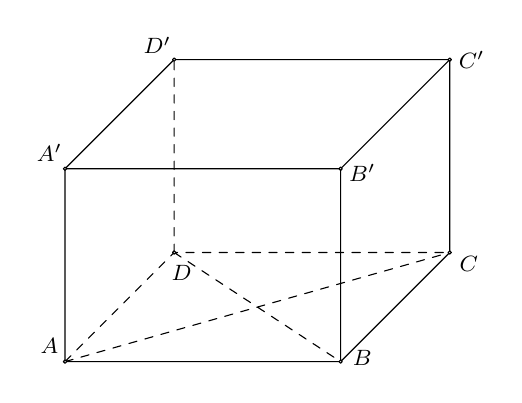
\begin{tikzpicture}[scale=0.7, font=\footnotesize,line join=round, line cap=round, >=stealth]
	\path
	(0:0) coordinate (D)
	(0:5) coordinate (C)
	(-135:2.8) coordinate (A)
	+(C) coordinate (B)
	\foreach \x in {A,B,C,D}{(\x)+(90:3.5) coordinate (\x')}
	;
	\draw[dashed] (A)--(D)--(C) (A)--(C) (D)--(B)(D)--(D');
	\draw 
	(A)--(B)--(B')--(A')--cycle
	(B)--(C)--(C')--(B')  (A')--(D')--(C')
	;
	\foreach \x/\g in {A/135,B/10,C/-30,D/-70,A'/135,B'/-10,C'/0,D'/140}\draw[fill=white] (\x) circle (.03) +(\g:.4) node{$\x$};
\end{tikzpicture}}	
		
		Các phương án còn lại:
		\begin{itemize}
			\item $(ABCD) \parallel (A'B'C'D')$ nên phương án $(ABCD) \perp (A'B'C'D')$ sai.
			\item Góc giữa $(A'BC)$ và $(ABCD)$ là góc $\widehat{A'BA} = 45^{\circ}$ nên phương án $(A'BC) \perp (ABCD)$ sai.
			\item Tương  phương án $(A'BC) \perp (A'B'C'D')$ sai.
		\end{itemize}
	}
\end{ex}

\begin{ex}%[2H5H2-2]%[Sở GD ĐT Cao Bằng]
	Trong không gian với hệ tọa độ $Oxyz$, cho đường thẳng $\Delta$ vuông góc với mặt phẳng $(\alpha)$ có phương trình $x + 2z + 3 = 0$. Một véc-tơ chỉ phương của đường thẳng $\Delta$ là
	\choice
	{$\vec{a} = (2;-1;0)$}
	{$\vec{a} = (2;0;-1)$}
	{\True $\vec{a} = (1;0;2)$}
	{$\vec{a} = (1;2;3)$}
	\loigiai{
		Mặt phẳng $(\alpha) \colon x + 2z + 3 = 0$ có một véc-tơ pháp tuyến là $\vec{n}_{(\alpha)} = (1; 0; 2)$.\\
		Vì đường thẳng $\Delta \perp (\alpha)$ nên đường thẳng $\Delta$ nhận véc-tơ pháp tuyến của mặt phẳng $(\alpha)$ làm véc-tơ chỉ phương.\\
		Vậy một véc-tơ chỉ phương của đường thẳng $\Delta$ là $\vec{u}_{\Delta} = \vec{n}_{(\alpha)} = (1; 0; 2)$.
	}
\end{ex}

\begin{ex}%[1H8H6-1]%[Sở GD ĐT Cao Bằng]
	Cho hình chóp $S.ABC$ có $SA$ vuông góc với mặt phẳng $(ABC)$, tam giác $ABC$ vuông cân tại $B$ và $SA = AB = a\sqrt{2}$. Góc giữa đường thẳng $SB$ và mặt phẳng $(ABC)$ bằng
	\choice
	{$90^{\circ}$}
	{\True $45^{\circ}$}
	{$30^{\circ}$}
	{$60^{\circ}$}
	\loigiai{
	\immini{	Vì $SA \perp (ABC)$ nên $A$ là hình chiếu vuông góc của $S$ lên mặt phẳng $(ABC)$.\\
		Suy ra $AB$ là hình chiếu vuông góc của $SB$ lên mặt phẳng $(ABC)$.\\
		Khi đó góc giữa đường thẳng $SB$ và mặt phẳng $(ABC)$ là góc $\widehat{SBA}$.\\
		Xét tam giác $SAB$ vuông tại $A$ có $SA = AB = a\sqrt{2}$ (giả thiết).\\
		Suy ra tam giác $SAB$ vuông cân tại $A$, do đó $\widehat{SBA} = 45^{\circ}$.\\
		Vậy góc giữa đường thẳng $SB$ và mặt phẳng $(ABC)$ bằng $45^{\circ}$.}{\begin{tikzpicture}[scale=0.6, font=\footnotesize,line join=round, line cap=round, >=stealth]
			\path
			(0,0) coordinate (A)
			(5,0) coordinate (C)
			(0,4) coordinate (S)
			(2,-2) coordinate (B)
			($(B)!0.3!(C)$) coordinate (H)
			;
			\foreach \x/\g in {A/135,B/-90,C/-10,S/90}\draw[fill=white] (\x) circle (.03) +(\g:.3) node{$\x$};
			
			\draw[thick] (S) -- (A)--(B)--(C)--cycle (S) -- (B) (S) -- (C) ; 
			\draw[dashed] (A) -- (C);
			\end{tikzpicture}}	
	
	}
\end{ex}

\begin{ex}%[1D6H4-3]%[Sở GD ĐT Cao Bằng]
	Tập nghiệm của bất phương trình $\log_4(x+1) \ge 2$ là
	\choice
	{$(-1; 15)$}
	{$(-1; 5]$}
	{\True $[15; +\infty)$}
	{$(15; +\infty)$}
	\loigiai{
		Điều kiện xác định: $x+1 > 0 \Leftrightarrow x > -1$.\\
		Vì cơ số $4 > 1$ nên bất phương trình đã cho tương đương với
		\begin{eqnarray*}
			& & x+1 \ge 4^2 \\
			&\Leftrightarrow & x+1 \ge 16 \\
			&\Leftrightarrow & x \ge 15.
		\end{eqnarray*}
		Kết hợp với điều kiện $x > -1$, ta được tập nghiệm của bất phương trình là $S = [15; +\infty)$.
	}
\end{ex}

\begin{ex}%[2D4H3-2]%[Sở GD ĐT Cao Bằng]
	Trong mặt phẳng với hệ tọa độ $Oxy$, cho hình phẳng $(H)$ giới hạn bởi các đường $y=x^2+3$, $y=0$, $x=0$, $x=2$. Gọi $V$ là thể tích khối tròn xoay được tạo thành khi quay $(H)$ xung quanh trục $Ox$. Mệnh đề nào sau đây đúng?
	\choice
	{\True $V = \pi \displaystyle\int\limits_{0}^{2} (x^2+3)^2 \mathrm{\,d}x$}
	{$V = \pi \displaystyle\int\limits_{0}^{2} (x^2+3) \mathrm{\,d}x$}
	{$V = \displaystyle\int\limits_{0}^{2} (x^2+3) \mathrm{\,d}x$}
	{$V = \displaystyle\int\limits_{0}^{2} (x^2+3)^2 \mathrm{\,d}x$}
	\loigiai{
		Thể tích khối tròn xoay khi quay hình phẳng $(H)$ giới hạn bởi các đường $y=f(x)$, trục $Ox$, đường thẳng $x=a$ và $x=b$ quanh trục $Ox$ được tính theo công thức:
		$$V = \pi \displaystyle\int\limits_{a}^{b} f^2(x) \mathrm{\,d}x.$$
		Áp dụng vào bài toán với $f(x)=x^2+3$, $a=0$ và $b=2$, ta có
		$$V = \pi \displaystyle\int\limits_{0}^{2} (x^2+3)^2 \mathrm{\,d}x.$$
	}
\end{ex}

\begin{ex}%[2D4H1-4]%[Sở GD ĐT Cao Bằng]
	Họ nguyên hàm của hàm số $f(x) = 2026^x$ là
	\choice
	{$\dfrac{2026^{x+1}}{\ln 2\,026} + C$}
	{\True $\dfrac{2026^x}{\ln 2\,026} + C$}
	{$2\,026^{x+1} + C$}
	{$2\,026^x + C$}
	\loigiai{
		Áp dụng công thức nguyên hàm cơ bản của hàm số mũ $\displaystyle\int a^x \mathrm{\,d}x = \dfrac{a^x}{\ln a} + C$ với $a = 2\,026$.\\
		Ta có $\displaystyle\int 2\,026^x \mathrm{\,d}x = \dfrac{2\,026^x}{\ln 2\,026} + C$.
	}
\end{ex}

\begin{ex}%[1D6H4-2]%[Sở GD ĐT Cao Bằng]
	Tổng các nghiệm của phương trình $\left(\dfrac{2}{3}\right)^{x^2-3x} = \dfrac{9}{4}$ là
	\choice
	{$0$}
	{$2$}
	{\True $3$}
	{$1$}
	\loigiai{
		Ta có $\dfrac{9}{4} = \left(\dfrac{3}{2}\right)^2 = \left(\dfrac{2}{3}\right)^{-2}$.\\
		Khi đó, phương trình đã cho tương đương với
		$$x^2 - 3x = -2 \Leftrightarrow x^2 - 3x + 2 = 0 \Leftrightarrow \hoac{&x=1\\&x=2.}$$
		Tổng các nghiệm của phương trình là $1 + 2 = 3$.
	}
\end{ex}

\begin{ex}%[2H2N1-1]%[Sở GD ĐT Cao Bằng]
	Cho hình hộp $ABCD.A'B'C'D'$. Vectơ $\vec{u} = \overrightarrow{A'A} + \overrightarrow{A'B'} + \overrightarrow{A'D'}$ bằng vectơ nào dưới đây?
	\choice
	{$\overrightarrow{CA'}$}
	{$\overrightarrow{C'A}$}
	{\True $\overrightarrow{A'C}$}
	{$\overrightarrow{AC'}$}
	\loigiai{
		Áp dụng quy tắc hình hộp cho hình hộp $ABCD.A'B'C'D'$, với ba cạnh xuất phát từ đỉnh $A'$ là $A'A$, $A'B'$ và $A'D'$. \\
		Theo quy tắc hình hộp, tổng của ba vectơ tương ứng với ba cạnh xuất phát từ một đỉnh của hình hộp bằng vectơ tương ứng với đường chéo của hình hộp xuất phát từ đỉnh đó. \\
		Do đó, $\overrightarrow{A'A} + \overrightarrow{A'B'} + \overrightarrow{A'D'} = \overrightarrow{A'C}$.
	}
\end{ex}

\begin{ex}%[1D1H5-3]%[Sở GD ĐT Cao Bằng]
	Tập nghiệm của phương trình $\cos 2x = 1$ là
	\choice
	{$\left\{ \dfrac{\pi}{2} + k2\pi, k \in \mathbb{Z} \right\}$}
	{\True $\left\{ k\pi, k \in \mathbb{Z} \right\}$}
	{$\left\{ k2\pi, k \in \mathbb{Z} \right\}$}
	{$\left\{ \dfrac{\pi}{4} + k\pi, k \in \mathbb{Z} \right\}$}
	\loigiai{
		Ta có phương trình lượng giác cơ bản
		$$\cos 2x = 1 \Leftrightarrow 2x = k2\pi \Leftrightarrow x = k\pi, k \in \mathbb{Z}.$$
		Vậy tập nghiệm của phương trình là $S = \{k\pi, k \in \mathbb{Z}\}$.
	}
\end{ex}

\begin{ex}%[1D5H2-3]%[Sở GD ĐT Cao Bằng]
	Khảo sát thời gian tập thể dục của một số học sinh khối $11$ thu được mẫu số liệu ghép nhóm sau:
	\begin{center}
		\begin{tabular}{|l|c|c|c|c|c|}
			\hline
			Thời gian (phút) & $[0; 20)$ & $[20; 40)$ & $[40; 60)$ & $[60; 80)$ & $[80; 100)$ \\
			\hline
			Số học sinh & $5$ & $9$ & $12$ & $10$ & $6$ \\
			\hline
		\end{tabular}
	\end{center}
	Nhóm chứa tứ phân vị thứ ba của mẫu số liệu ghép nhóm trên là
	\choice
	{$[40; 60)$}
	{$[20; 40)$}
	{\True $[60; 80)$}
	{$[80; 100)$}
	\loigiai{
		Tổng số học sinh (cỡ mẫu) là $n = 5 + 9 + 12 + 10 + 6 = 42$.\\
		Vị trí của tứ phân vị thứ ba $Q_3$ trong mẫu số liệu gốc là $\dfrac{3n}{4} = \dfrac{3 \cdot 42}{4} = 31{,}5$.\\
		Ta có bảng tần số tích lũy:
		\begin{itemize}
			\item Nhóm $[0; 20)$ có tần số tích lũy là $5$.
			\item Nhóm $[20; 40)$ có tần số tích lũy là $5 + 9 = 14$.
			\item Nhóm $[40; 60)$ có tần số tích lũy là $14 + 12 = 26$.
			\item Nhóm $[60; 80)$ có tần số tích lũy là $26 + 10 = 36$.
		\end{itemize}
		Vì $26 < 31{,}5 < 36$ nên giá trị tứ phân vị thứ ba $Q_3$ thuộc nhóm $[60; 80)$.
	}
\end{ex}

\begin{ex}%[1D2H3-4]%[Sở GD ĐT Cao Bằng]
	Cho cấp số nhân $(u_n)$ với $u_1 = 2$ và công bội $q = 3$. Giá trị của $u_4$ bằng
	\choice
	{$162$}
	{$24$}
	{$48$}
	{\True $54$}
	\loigiai{
		Số hạng tổng quát của cấp số nhân $(u_n)$ là $u_n = u_1 \cdot q^{n-1}$.\\
		Áp dụng với $n=4$, ta có
		$$u_4 = u_1 \cdot q^3 = 2 \cdot 3^3 = 2 \cdot 27 = 54.$$
		Vậy giá trị của $u_4$ bằng $54$.
	}
\end{ex}

%%%==============HetCau_EX12==============%%%

\Closesolutionfile{ans}
\indapan{12}{ans/SoGDCaoBang-phan1}


%%%------------PHẦN 2-------------------
\cauds
\Opensolutionfile{ans}[ans/SoGDCaoBang-phan2]
%%%%==============Cau_EX1==============%%%

\begin{ex}%[2D4V1-6]%[Sở GD ĐT Cao Bằng]
	Trong quá trình sản xuất giấy, việc kiểm soát bọt rất quan trọng để đảm bảo chất lượng sản phẩm. Giả sử $y(x)$ là nồng độ của một chất gây bọt còn dư trong bể xử lý (đơn vị $\mathrm{mol/L}$) tại thời điểm $x$ (giây), $y(x) > 0$ với $x \ge 0$. Sau khi thêm một lượng chất chống tạo bọt, nồng độ chất gây bọt giảm dần theo thời gian thỏa mãn hệ thức $y'(x) = -7 \cdot 10^{-4} y(x)$ với $x \ge 0$. Biết rằng tại thời điểm bắt đầu xử lý $x = 0$, nồng độ chất gây bọt là $0{,}05 \mathrm{~mol/L}$. Xét hàm số $f(x) = \ln y(x)$ với $x \ge 0$.
	\choiceTF
	{\True $f'(x) = -7 \cdot 10^{-4}$}
	{\True $f(x) = -7 \cdot 10^{-4} x + \ln(0{,}05)$}
	{$y(30) - y(15) \approx 5{,}7 \cdot 10^{-4}$}
	{Nồng độ trung bình của chất gây bọt trong khoảng thời gian từ giây thứ $20$ đến giây thứ $30$ bằng $0{,}03 \mathrm{~mol/L}$}
	\loigiai{
		Từ hệ thức $y'(x) = -7 \cdot 10^{-4} y(x) \Rightarrow \dfrac{y'(x)}{y(x)} = -7 \cdot 10^{-4}$.\\
		Lấy nguyên hàm hai vế ta có $\displaystyle\int \dfrac{y'(x)}{y(x)} \mathrm{d}x = \displaystyle\int -7 \cdot 10^{-4} \mathrm{d}x \Rightarrow \ln y(x) = -7 \cdot 10^{-4} x + C$.\\
		Tại $x = 0$, $y(0) = 0{,}05 \Rightarrow \ln(0{,}05) = C$.
		\begin{itemchoice}
			\itemch Ta có $f(x) = \ln y(x) = -7 \cdot 10^{-4} x + \ln(0{,}05) \Rightarrow f'(x) = -7 \cdot 10^{-4}$.
			\itemch  $f(x) = -7 \cdot 10^{-4} x + \ln(0{,}05)$.
			\itemch Ta có $y(x) = \mathrm{e}^{f(x)} = 0{,}05 \cdot \mathrm{e}^{-7 \cdot 10^{-4} x}$.\\
			$y(30) - y(15) = 0{,}05 \cdot \left( \mathrm{e}^{-7 \cdot 10^{-4} \cdot 30} - \mathrm{e}^{-7 \cdot 10^{-4} \cdot 15} \right) \approx -5{,}17 \cdot 10^{-4}$.
			\itemch Nồng độ trung bình được tính theo công thức:\\
			$\overline{y} = \dfrac{1}{30 - 20} \displaystyle\int\limits_{20}^{30} 0{,}05 \cdot \mathrm{e}^{-7 \cdot 10^{-4} x} \mathrm{\,d}x = \dfrac{0{,}05}{10} \left[ \dfrac{\mathrm{e}^{-7 \cdot 10^{-4} x}}{-7 \cdot 10^{-4}} \right]_{20}^{30} \approx 0{,}049 \mathrm{~mol/L} \ne 0{,}03$.
		\end{itemchoice}
	}
\end{ex}

\begin{ex}%[2D6V2-4]%[Sở GD ĐT Cao Bằng]
	An và Bình là bạn thân ngồi cùng bàn. Cả hai đều có thói quen chuẩn bị sẵn nhiều bút bi mực xanh và bút bi mực đen (tất cả đều còn mực) trong hộp bút của mình. Cả hai bạn cùng dùng loại bút bi E178 giống nhau.
	Trong hộp bút của An chỉ có $10$ chiếc bút bi E178 gồm: $5$ bút bi mực xanh và $5$ bút bi mực đen.
	Trong hộp bút của Bình chỉ có $10$ chiếc bút bi E178 gồm: $6$ bút bi mực xanh và $4$ bút bi mực đen.
	An lấy ngẫu nhiên $1$ chiếc bút bi từ hộp của mình bỏ vào hộp của Bình. Sau đó, Bình lấy ngẫu nhiên từ hộp của mình ra $1$ chiếc bút bi để làm bài tập.
	\choiceTF
	{Xác suất để chiếc bút bi An bỏ vào hộp của Bình là bút bi mực xanh bằng $\dfrac{6}{11}$}
	{\True Xác suất để chiếc bút bi Bình lấy ra từ hộp của mình là chiếc bút bi của An bằng $\dfrac{1}{11}$}
	{\True Xác suất để chiếc bút bi Bình lấy ra từ hộp của mình là bút bi mực xanh bằng $\dfrac{13}{22}$}
	{\True Giả sử Bình lấy ra được một chiếc bút bi mực xanh từ hộp của mình. Xác suất để chiếc bút bi đó vốn thuộc về hộp của An ban đầu bằng $\dfrac{1}{13}$}
	\loigiai{
		Gọi $A$ là biến cố: \lq\lq An lấy được bút xanh bỏ vào hộp Bình\rq\rq.\\
		Gọi $B$ là biến cố: \lq\lq Bình lấy ra được bút mực xanh từ hộp của mình\rq\rq.
		\begin{center}
			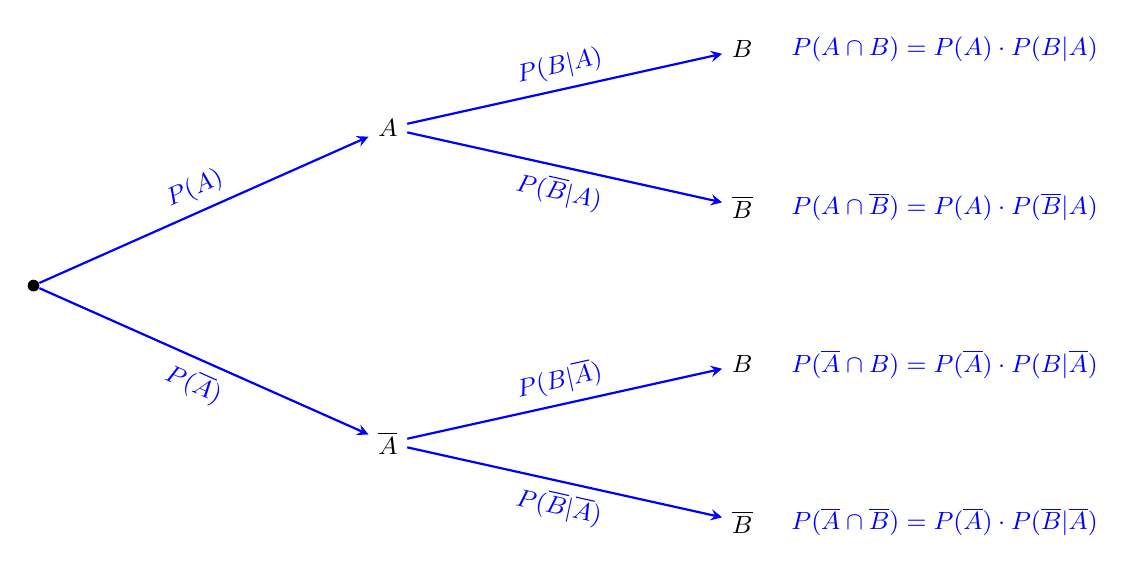
\begin{tikzpicture}[
				grow=right,
				sloped,
				level 1/.style={sibling distance=4cm, level distance=4.5cm},
				level 2/.style={sibling distance=2cm, level distance=4.5cm},
				edge from parent/.style={draw, ->, >=stealth, blue, thick},
				every node/.style={text=blue, font=\small}
				]
				
				% Gốc sơ đồ
				\node[circle, fill=black, inner sep=1.5pt] (root) {}
				child {
					node[black] (notA) {$\overline{A}$}
					child {
						node[black] (notAnotB) {$\overline{B}$}
						edge from parent node[below] {$P(\overline{B}|\overline{A})$}
					}
					child {
						node[black] (notAB) {$B$}
						edge from parent node[above] {$P(B|\overline{A})$}
					}
					edge from parent node[below] {$P(\overline{A})$}
				}
				child {
					node[black] (A) {$A$}
					child {
						node[black] (AnotB) {$\overline{B}$}
						edge from parent node[below] {$P(\overline{B}|A)$}
					}
					child {
						node[black] (AB) {$B$}
						edge from parent node[above] {$P(B|A)$}
					}
					edge from parent node[above] {$P(A)$}
				};
				
				% Cột công thức kết quả cuối cùng
				\begin{scope}[xshift=9.5cm]
					\node[anchor=west] at (0, 3)  {$P(A \cap B) = P(A) \cdot P(B|A)$};
					\node[anchor=west] at (0, 1)  {$P(A \cap \overline{B}) = P(A) \cdot P(\overline{B}|A)$};
					\node[anchor=west] at (0, -1) {$P(\overline{A} \cap B) = P(\overline{A}) \cdot P(B|\overline{A})$};
					\node[anchor=west] at (0, -3) {$P(\overline{A} \cap \overline{B}) = P(\overline{A}) \cdot P(\overline{B}|\overline{A})$};
				\end{scope}
				
			\end{tikzpicture}
		\end{center}
		\begin{itemchoice}
			\itemch Ta có hộp của An có $5$ bút xanh và $5$ bút đen.\\ Xác suất để An lấy được bút xanh là $\mathrm{P}(A) = \dfrac{5}{10} = \dfrac{1}{2}$.
			\itemch Sau khi An bỏ $1$ chiếc bút vào hộp của Bình, hộp của Bình có tổng cộng $10 + 1 = 11$ chiếc bút.\\ Xác suất để Bình lấy đúng chiếc bút mà An vừa bỏ vào là $\dfrac{1}{11}$.
			\itemch Ta tính xác suất của biến cố $B$ bằng công thức xác suất toàn phần:\\
			$\mathrm{P}(B) = \mathrm{P}(A) \cdot \mathrm{P}(B|A) + \mathrm{P}(\overline{A}) \cdot \mathrm{P}(B|\overline{A})$.
			\begin{itemize}
				\item Nếu $A$ xảy ra: An bỏ $1$ bút xanh vào, hộp Bình có $7$ xanh, $4$ đen $\Rightarrow \mathrm{P}(B|A) = \dfrac{7}{11}$.
				\item  Nếu $\overline{A}$ xảy ra: An bỏ $1$ bút đen vào, hộp Bình có $6$ xanh, $5$ đen $\Rightarrow \mathrm{P}(B|\overline{A}) = \dfrac{6}{11}$.
			\end{itemize}
			Vậy $\mathrm{P}(B) = \dfrac{1}{2} \cdot \dfrac{7}{11} + \dfrac{1}{2} \cdot \dfrac{6}{11} = \dfrac{13}{22}$.
			\itemch Đây là xác suất có điều kiện (Công thức Bayes).\\
			Gọi $E$ là biến cố chiếc bút Bình lấy ra là của An.
			 Ta cần tính xác suất để chiếc bút Bình lấy ra thuộc về An ($E$) với điều kiện đó là bút xanh ($B$).\\
			 Ta có 	$\mathrm{P}(E|B) = \dfrac{\mathrm{P}(E \cap B)}{\mathrm{P}(B)}$.\\
			Biến cố $(E \cap B)$ xảy ra khi An bỏ bút xanh vào hộp Bình $\left(\text{xác suất bằng}\,\,  \dfrac{1}{2}\right)$ và Bình lấy đúng chiếc bút đó $\left(\text{xác suất bằng}\,\, \dfrac{1}{11}\right)$.\\
			$\Rightarrow \mathrm{P}(E \cap B) = \dfrac{1}{2} \cdot \dfrac{1}{11} = \dfrac{1}{22}$.\\
			$\Rightarrow \mathrm{P}(E|B) = \dfrac{1/22}{13/22} = \dfrac{1}{13}$.
		\end{itemchoice}
	}
\end{ex}

\begin{ex}%[2D1H4-4]%[Sở GD ĐT Cao Bằng]
	Cho hàm số $y=f(x)=\dfrac{x^2+4x-1}{x-1}$.
	\choiceTF
	{\True Hàm số đã cho có tập xác định là $\mathscr{D}=\mathbb{R}\setminus\{1\}$}
	{\True Hàm số đã cho có đạo hàm là $f'(x)=\dfrac{x^2-2x-3}{(x-1)^2}$}
	{Giá trị nhỏ nhất của hàm số $f(x)$ trên đoạn $[2;3]$ bằng $7$}
	{\True Phương trình đường tiệm cận xiên của đồ thị hàm số $f(x)$ là $y=x+5$}
	\loigiai{
		\begin{itemchoice}
			\itemch Điều kiện xác định: $x-1 \neq 0 \Leftrightarrow x \neq 1$. Vậy tập xác định $\mathscr{D}=\mathbb{R}\setminus\{1\}$.
			\itemch Ta có 
				\begin{eqnarray*}
				f'(x)&  =&  \dfrac{(x^2+4x-1)'(x-1) - (x^2+4x-1)(x-1)'}{(x-1)^2}\\
				& =&  \dfrac{(2x+4)(x-1) - (x^2+4x-1)}{(x-1)^2}\\
				& =&   \dfrac{x^2-2x-3}{(x-1)^2}.
			\end{eqnarray*}
		
			\itemch Xét $f'(x)=0 \Leftrightarrow x^2-2x-3=0 \Leftrightarrow \hoac{&x=-1 \notin [2;3] \\ &x=3 \in [2;3].}$ \\
			Tính các giá trị: $f(2) = \dfrac{2^2+4 \cdot 2 - 1}{2-1} = 11$; $f(3) = \dfrac{3^2+4 \cdot 3 - 1}{3-1} = 10$. \\
			Vậy $\min\limits_{x \in [2;3]} f(x) = 10$ tại $x=3$.
			\itemch Ta có	 $y = \dfrac{x^2+4x-1}{x-1} = \dfrac{x(x-1) + 5(x-1) + 4}{x-1} = x + 5 + \dfrac{4}{x-1}$. \\
			Vì $\displaystyle\lim\limits_{x \to \pm\infty} \left[f(x) - (x+5)\right] = \displaystyle\lim\limits_{x \to \pm\infty} \dfrac{4}{x-1} = 0$, nên đường thẳng $y=x+5$ là tiệm cận xiên của đồ thị hàm số.
		\end{itemchoice}
	}
\end{ex}

\begin{ex}%[2H5V2-8]%[Sở GD ĐT Cao Bằng]
	Trong không gian với hệ tọa độ $Oxyz$ (đơn vị đo trên các trục là km), một máy bay phản lực đang bay thẳng theo lộ trình $\Delta$ là đường thẳng có phương trình $\Delta \colon \dfrac{x-50}{3} = \dfrac{y+20}{-4} = \dfrac{z-10}{1}$. Radar tại trạm kiểm soát không lưu phát hiện một khối mây dông tích điện nguy hiểm có dạng hình cầu $(S)$ với tâm $C(200;-300;60)$ và bán kính $R=80$ km. Tại thời điểm quan sát, máy bay đang ở vị trí $A(50;-20;10) \in \Delta$.
	\choiceTF
	{Một vectơ chỉ phương của đường thẳng $\Delta$ là $\vec{u}=(5;-2;1)$}
	{\True Đường thẳng $\Delta$ nằm trong mặt phẳng $(P) \colon 4x+3y=140$}
	{\True Nếu tiếp tục giữ nguyên lộ trình $\Delta$ thì máy bay phản lực sẽ bay xuyên qua (bay vào bên trong) khối mây dông có dạng hình cầu $(S)$}
	{\True Gọi $M$ là điểm trên đường thẳng $\Delta$ mà tại đó máy bay phản lực gần tâm $C$ của hình cầu $(S)$ nhất. Biết rằng tốc độ máy bay phản lực không đổi là $500$ km/h. Thời gian máy bay phản lực đó di chuyển từ vị trí điểm $A$ đến điểm $M$ nhỏ hơn $30$ phút}
	\loigiai{
		\begin{itemchoice}
			\itemch Từ phương trình chính tắc của đường thẳng $\Delta \colon \dfrac{x-50}{3} = \dfrac{y+20}{-4} = \dfrac{z-10}{1}$, ta có một vectơ chỉ phương là $\vec{u}_{\Delta}=(3;-4;1)$. Vectơ $(5;-2;1)$ không cùng phương với $\vec{u}_{\Delta}$.
			\itemch Kiểm tra $A(50;-20;10) \in (P)$: $4(50) + 3(-20) = 200 - 60 = 140$ (đúng).\\
			Vectơ pháp tuyến của $(P)$ là $\vec{n}_P=(4;3;0)$. Ta có $\vec{u}_{\Delta} \cdot \vec{n}_P = 3 \cdot 4 + (-4) \cdot 3 + 1 \cdot 0 = 0$. Vậy $\Delta \subset (P)$.
			\itemch Ta tính khoảng cách từ tâm $C(200;-300;60)$ đến lộ trình $\Delta$.\\
			Điểm $A(50;-20;10) \in \Delta$, $\overrightarrow{AC}=(150;-280;50)$. Vectơ chỉ phương $\vec{u}_{\Delta}=(3;-4;1)$.\\
			$\left[ \overrightarrow{AC}, \vec{u}_{\Delta} \right] = (-80; 0; 240)$.\\
			$\mathrm{d}(C, \Delta) = \dfrac{\left| \left[ \overrightarrow{AC}, \vec{u}_{\Delta} \right] \right|}{\left| \vec{u}_{\Delta} \right|} = \dfrac{\sqrt{(-80)^2 + 0^2 + 240^2}}{\sqrt{3^2 + (-4)^2 + 1^2}} = \dfrac{80\sqrt{10}}{\sqrt{26}} \approx 49{,}6$ km.\\
			Vì $\mathrm{d}(C, \Delta) \approx 49{,}6 < R = 80$ nên lộ trình $\Delta$ cắt khối mây hình cầu $(S)$.
			\itemch Điểm $M$ là hình chiếu của $C$ lên $\Delta$. Gọi $M(50+3t; -20-4t; 10+t) \in \Delta$.\\
			$\overrightarrow{CM} = (3t-150; -4t+280; t-50)$.\\
			Vì $CM \perp \Delta \Leftrightarrow \overrightarrow{CM} \cdot \vec{u}_{\Delta} = 0 \Leftrightarrow 3(3t-150) - 4(-4t+280) + 1(t-50) = 0 \Leftrightarrow 26t = 1620 \Leftrightarrow t = \dfrac{810}{13}$.\\
			Khoảng cách $AM = \sqrt{(3t)^2 + (-4t)^2 + t^2} = |t|\sqrt{26} = \dfrac{810}{13} \cdot \sqrt{26} \approx 158{,}85$ km.\\
			Thời gian di chuyển: $T = \dfrac{AM}{v} = \dfrac{158{,}85}{500} \approx 0{,}3177$ giờ $\approx 19{,}06$ phút.\\
			Vậy thời gian nhỏ hơn $30$ phút là đúng.
		\end{itemchoice}
	}
\end{ex}

%%%%==============HetCau_EX4==============%%%
\Closesolutionfile{ans}
\indapan{2}{ans/SoGDCaoBang-phan2}



%%%------------PHẦN 3-------------------

\caukq
\Opensolutionfile{ans}[ans/SoGDCaoBang-phan3]
%%%%==============Cau_EX1==============%%%
\begin{ex}%[1D2C2-2]%[Sở GD ĐT Cao Bằng]
\immini{	Cho một hình bát giác đều $ABCDEFGH$ nội tiếp trong một đường tròn tâm $O$ như hình bên. Gắn ngẫu nhiên tám số tự nhiên $\{9; 10; 11; 12; 13; 14; 15; 16\}$ vào tám đỉnh của bát giác đều này (mỗi số gắn đúng một đỉnh). Chọn ngẫu nhiên một tam giác có ba đỉnh lấy từ tám đỉnh của bát giác đã cho. Gọi xác suất để thu được một tam giác vuông với ba số trên ba đỉnh của tam giác (theo một thứ tự nào đó) lập thành một cấp số cộng là $\dfrac{m}{n}$ ($m, n \in \mathbb{N}^*$; $\dfrac{m}{n}$ là phân số tối giản). Giá trị của $m+n$ bằng bao nhiêu?
	\shortans{107}}{\begin{tikzpicture}[line join=round, line cap=round, >=Stealth, font=\footnotesize]|
		% 1. Định nghĩa các tham số
		\def\R{3} % Bán kính đường tròn ngoại tiếp
		\coordinate (O) at (0,0);
		
		% 2. Vẽ vòng tròn ngoại tiếp
		\draw[thick] (O) circle (\R);
		
		% 3. Xác định tọa độ các đỉnh từ A đến H theo vòng tròn (mỗi bước 45 độ)
		% Bắt đầu từ góc 20 độ để hình trông cân đối như trong ảnh mẫu
		\foreach \i/\label in {0/A, 1/B, 2/C, 3/D, 4/E, 5/F, 6/G, 7/H} {
			\coordinate (\label) at ({20 + \i*45}:\R);
		}
		
		% 4. Tô màu nền các tam giác (tạo hiệu ứng mảng xám nhạt như ảnh)
		\fill[gray!10] (A) -- (B) -- (C) -- (D) -- (E) -- (F) -- (G) -- (H) -- cycle;
		
		% 5. Vẽ các đường nối từ tâm O đến các đỉnh
		\foreach \p in {A,B,C,D,E,F,G,H} {
			\draw[thin, black!60] (O) -- (\p);
		}
		
		% 6. Vẽ các cạnh của đa giác
		\draw[thick] (A) -- (B) -- (C) -- (D) -- (E) -- (F) -- (G) -- (H) -- cycle;
		
		% 7. Vẽ các điểm (nodes) và dán nhãn
		\fill (O) circle (2pt) node[above right=-1pt] {$O$};
		
		\foreach \p/\pos in {A/right, B/above right, C/above, D/above left, E/left, F/below left, G/below, H/below right} {
			\fill (\p) circle (2pt);
			\node[\pos] at (\p) {$\p$};
		}
		
		\end{tikzpicture}}	

	\loigiai{
Gọi $\Omega$ là không gian mẫu của việc chọn ngẫu nhiên $3$ đỉnh từ $8$ đỉnh và gán ngẫu nhiên $8$ số vào $8$ đỉnh. Ta có thể tính xác suất thông qua hai biến cố độc lập:
\begin{itemize}
	\item Biến cố $A$: \lq\lq Chọn được một tam giác vuông từ các đỉnh của bát giác đều\rq\rq.
	\item Biến cố $B$: \lq\lq Ba số trên ba đỉnh được chọn lập thành một cấp số cộng\rq\rq.
\end{itemize}
\textbf{1. Tính xác suất của biến cố $A$:}
\begin{itemize}
	\item Số cách chọn $3$ đỉnh từ $8$ đỉnh của bát giác là $n(\Omega_A) = \mathrm{C}_8^3 = 56$.
	\item Một tam giác nội tiếp đường tròn là tam giác vuông khi và chỉ khi có một cạnh là đường kính. Bát giác đều có $4$ đường kính. Mỗi đường kính kết hợp với một trong $6$ đỉnh còn lại tạo thành một tam giác vuông.
	\item Số tam giác vuông là $4 \cdot 6 = 24$.
	\item Suy ra $\mathrm{P}(A) = \dfrac{24}{56} = \dfrac{3}{7}$.
\end{itemize}
\textbf{2. Tính xác suất của biến cố $B$:}
\begin{itemize}
	\item Việc gán $8$ số vào $8$ đỉnh và chọn $3$ đỉnh tương đương với việc chọn ngẫu nhiên $3$ số từ tập $S = \{9; 10; 11; 12; 13; 14; 15; 16\}$.
	\item Số cách chọn $3$ số từ $8$ số là $n(\Omega_B) = \mathrm{C}_8^3 = 56$.
	\item Các bộ $3$ số $(a, b, c)$ với $a < b < c$ lập thành cấp số cộng ($a+c=2b$):
	\begin{itemize}
		\item Công sai $d=1$: $\{9, 10, 11\}, \{10, 11, 12\}, \{11, 12, 13\}, \{12, 13, 14\}, \{13, 14, 15\}, \{14, 15, 16\}$ (có $6$ bộ).
		\item Công sai $d=2$: $\{9, 11, 13\}, \{10, 12, 14\}, \{11, 13, 15\}, \{12, 14, 16\}$ (có $4$ bộ).
		\item Công sai $d=3$: $\{9, 12, 15\}, \{10, 13, 16\}$ (có $2$ bộ).
	\end{itemize}
	\item Tổng số bộ số thỏa mãn là $6 + 4 + 2 = 12$ bộ.
	\item Suy ra $\mathrm{P}(B) = \dfrac{12}{56} = \dfrac{3}{14}$.
\end{itemize}
\textbf{3. Tính xác suất của bài toán:}
\begin{itemize}
	\item Vì biến cố $A$ và $B$ độc lập nên xác suất cần tìm là:
	$$\mathrm{P} = \mathrm{P}(A) \cdot \mathrm{P}(B) = \dfrac{3}{7} \cdot \dfrac{3}{14} = \dfrac{9}{98}.$$
	\item Do $\dfrac{9}{98}$ là phân số tối giản nên $m = 9$ và $n = 98$.
	\item Vậy $m + n = 9 + 98 = 107$.
\end{itemize}
	}
\end{ex}

\begin{ex}%[1H8V7-3]%[Sở GD ĐT Cao Bằng]
	Cho hình chóp $S.ABCD$ có đáy $ABCD$ là hình vuông, cạnh bên $SA$ vuông góc với mặt phẳng đáy, tam giác $SBD$ là tam giác đều, $SA=a\sqrt{2}$. Thể tích của khối chóp $S.ABCD$ là $V_{S.ABCD} = \dfrac{m\sqrt{2} \cdot a^3}{n}$ ($m, n \in \mathbb{N}^*$; $\dfrac{m}{n}$ là phân số tối giản). Giá trị $m + 2026n$ bằng bao nhiêu?
	\shortans{6080}
	\loigiai{
		\immini{
			Gọi $x$ là độ dài cạnh của hình vuông $ABCD$ ($x > 0$).\\
			Vì $ABCD$ là hình vuông cạnh $x$ nên đường chéo $BD = x\sqrt{2}$.\\
			Xét tam giác $SAB$ vuông tại $A$, ta có $SB^2 = SA^2 + AB^2 = (a\sqrt{2})^2 + x^2 = 2a^2 + x^2$.\\
			Theo giả thiết, tam giác $SBD$ đều nên $SB = BD$.\\
			Suy ra $SB^2 = BD^2 \Leftrightarrow 2a^2 + x^2 = (x\sqrt{2})^2$\\
			$\Leftrightarrow 2a^2 + x^2 = 2x^2 \Leftrightarrow x^2 = 2a^2 \Leftrightarrow x = a\sqrt{2}$.\\
			Diện tích đáy $ABCD$ là $S_{ABCD} = x^2 = 2a^2$.
		}{
			\begin{tikzpicture}[scale=0.7, font=\footnotesize, line join=round, line cap=round, >=stealth]
				\coordinate (A) at (0,0);
				\coordinate (B) at (4,0);
				\coordinate (D) at (-1.5,-1.5);
				\coordinate (C) at ($(B)+(D)-(A)$);
				\coordinate (S) at (0,4);
				\draw (S)--(D)--(C)--(B)--(S)--(C);
				\draw[dashed] (S)--(A)--(B) (A)--(D) (S)--(B) (B)--(D);
				\fill[black] (S) circle (1.5pt) node[above] {$S$};
				\fill[black] (A) circle (1.5pt) node[above right] {$A$};
				\fill[black] (B) circle (1.5pt) node[right] {$B$};
				\fill[black] (C) circle (1.5pt) node[below] {$C$};
				\fill[black] (D) circle (1.5pt) node[left] {$D$};
				\draw (0,0.3)--(0.3,0.3)--(0.3,0);
			\end{tikzpicture}
		}
		Thể tích khối chóp $S.ABCD$ là
		$$V_{S.ABCD} = \dfrac{1}{3} \cdot S_{ABCD} \cdot SA = \dfrac{1}{3} \cdot 2a^2 \cdot a\sqrt{2} = \dfrac{2\sqrt{2} \cdot a^3}{3}.$$
		Đối chiếu với công thức $V_{S.ABCD} = \dfrac{m\sqrt{2} \cdot a^3}{n}$, ta được $m = 2$ và $n = 3$.\\
		Vì $\dfrac{2}{3}$ là phân số tối giản và $2, 3 \in \mathbb{N}^*$ nên thỏa mãn điều kiện bài toán.\\
		Giá trị của biểu thức $m + 2\,026n = 2 + 2\,026 \cdot 3 = 2 + 6\,078 = 6\,080$.
	}
\end{ex}

\begin{ex}%[0D8V2-9]%[Sở GD ĐT Cao Bằng]
	Trong giải cờ vua giao hữu tại một trường THPT chào mừng ngày thành lập Đoàn 26/3, các vận động viên nam và nữ cùng tham gia thi đấu. Để đảm bảo tính công bằng, giúp mỗi kỳ thủ đều được cầm quân Trắng và quân Đen khi đối đầu với các đối thủ khác thì Ban tổ chức quy định thể thức thi đấu vòng tròn hai lượt tức là mỗi cặp vận động viên sẽ thi đấu với nhau đúng $2$ ván. Biết rằng giải chỉ có $2$ vận động viên nữ tham gia. Sau khi kết thúc giải, Ban tổ chức thống kê được số ván các vận động viên nam thi đấu với nhau nhiều hơn số ván họ thi đấu với các vận động viên nữ là $66$ ván. Hỏi tổng số ván mà tất cả các vận động viên đã thi đấu là bao nhiêu?
	\shortans{156}
	\loigiai{
		Gọi $n$ là tổng số vận động viên tham gia giải ($n > 2, n \in \mathbb{N}$).\\
		Vì có $2$ vận động viên nữ nên số vận động viên nam là $n-2$.\\
		Theo thể thức thi đấu vòng tròn hai lượt, mỗi cặp đấu với nhau $2$ ván, ta có:
		\begin{itemize}
			\item Số ván các vận động viên nam thi đấu với nhau là $2 \cdot \mathrm{C}_{n-2}^2 = (n-2)(n-3)$ ván.
			\item Số ván các vận động viên nam thi đấu với các vận động viên nữ là $2 \cdot (n-2) \cdot 2 = 4(n-2)$ ván.
		\end{itemize}
		Theo giả thiết, ta có phương trình:
		\begin{eqnarray*}
			& & (n-2)(n-3) - 4(n-2) = 66 \\
			&\Leftrightarrow & (n-2)(n-3-4) = 66 \\
			&\Leftrightarrow & (n-2)(n-7) = 66 \\
			&\Leftrightarrow & n^2 - 9n + 14 = 66 \\
			&\Leftrightarrow & n^2 - 9n - 52 = 0 \\
			&\Leftrightarrow & \hoac{&n = 13 \text{ (nhận)} \\ &n = -4 \text{ (loại).}}
		\end{eqnarray*}
		Vậy tổng số vận động viên tham gia là $13$ người.\\
		Tổng số ván mà tất cả các vận động viên đã thi đấu là $2 \cdot \mathrm{C}_{13}^2 = 13 \cdot 12 = 156$ ván.
	}
\end{ex}

\begin{ex}%[2D1V3-6]%[Sở GD ĐT Cao Bằng]
	Một doanh nghiệp dự định sản xuất $x$ sản phẩm trong một tháng ($x \in \mathbb{N}; 100 \le x \le 800$). Tổng doanh thu khi bán hết $x$ sản phẩm đó là $F(x)=-0{,}001x^3 + 0{,}6x^2 + 500x + 100\,000$ (nghìn đồng). Chi phí để sản xuất bình quân cho mỗi sản phẩm là $G(x) = 0{,}0002x^2 + \dfrac{40\,000}{x}$ (nghìn đồng) và chi phí để mua nguyên vật liệu khi chưa chiết khấu là $H(x) = \dfrac{-4}{49}x^2 + \dfrac{750}{49}x + \dfrac{1\,500\,000}{49}$ (nghìn đồng). Do được giảm $2\%$ tổng tiền mua nguyên vật liệu, hãy tìm số sản phẩm $x$ để lợi nhuận thu được là lớn nhất.
	\shortans{602}
	\loigiai{
		\begin{itemize}
			\item Tổng chi phí sản xuất cố định: $C_1(x) = x \cdot G(x) = 0{,}0002x^3 + 40\,000$.
			\item Chi phí mua nguyên vật liệu thực tế sau khi giảm $2\%$:
			$$C_2(x) = 0{,}98 \cdot \left(\dfrac{-4}{49}x^2 + \dfrac{750}{49}x + \dfrac{1\,500\,000}{49}\right) = -0{,}08x^2 + 15x + 30\,000.$$
			\item Hàm lợi nhuận của doanh nghiệp là:
			\begin{eqnarray*}
				L(x) &=& F(x) - C_1(x) - C_2(x) \\
				&=& (-0{,}001x^3 + 0{,}6x^2 + 500x + 100\,000) - (0{,}0002x^3 + 40\,000) - (-0{,}08x^2 + 15x + 30\,000) \\
				&=& -0{,}0012x^3 + 0{,}68x^2 + 485x + 30\,000.
			\end{eqnarray*}
			\item Xét đạo hàm trên $[100; 800]$: $L'(x) = -0{,}0036x^2 + 1{,}36x + 485$.
			\item $L'(x) = 0 \Leftrightarrow \heva{&x \approx 601{,}67 \\ &x \approx -223{,}89 \text{ (loại).}}$
			\item Ta có bảng biến thiên: $L'(x)$ đổi dấu từ dương sang âm khi đi qua $x \approx 601{,}67$. 
			\begin{center}
				\begin{tikzpicture}
					\tkzTabInit[nocadre=false, lgt=1.4, espcl=3.8, deltacl=0.6]
					{$x$ /0.8, $L'(x)$ /0.8, $L(x)$ /2}
					{100, $601{,}67$, 800}
					\tkzTabLine{ , +, 0, -, }
					\tkzTabVar{-/ $84\,100$, +/ $\text{CĐ}$, -/ $233\,200$}
				\end{tikzpicture}
			\end{center}
			\item Vì $x \in \mathbb{N}$, so sánh $L(601)$ và $L(602)$:
			\begin{itemize}
				\item $L(601) = -0{,}0012(601)^3 + 0{,}68(601)^2 + 485\,601 + 30\,000 \approx 307\,232{,}11$.
				\item $L(602) = -0{,}0012602^3 + 0{,}68(602)^2 + 485\,602 + 30\,000 \approx 307\,233{,}15$.
			\end{itemize}
			\item Vậy doanh nghiệp cần sản xuất $602$ sản phẩm để lợi nhuận thu được là lớn nhất.
		\end{itemize}
	}
\end{ex}


\begin{ex}%[2H5C2-6]%[Sở GD ĐT Cao Bằng]
\immini{	Trong bản thiết kế của dự án lắp đặt đường dây điện cho vùng núi tỉnh $A$, các kĩ sư dự kiến xây dựng các trụ điện cao $120$ m. Để giữ thăng bằng cho trụ điện, hệ thống dây cáp được nối từ đỉnh trụ $S$ xuống mặt đất giả định tại các điểm $A, B, C$ trên mặt phẳng nằm ngang sao cho $S.ABC$ là hình chóp tam giác đều, khoảng cách từ chân trụ đến các điểm $A, B, C$ bằng $40\sqrt{3}$ m. Tuy nhiên, do địa hình thực tế là sườn núi dốc $10^{\circ}$ nên vị trí tiếp đất thực tế của dây cáp sẽ tại $A, B', C'$ ($BB', CC'$ song song với thân trụ điện).}{	\begin{tikzpicture}[scale=0.7, font=\footnotesize,line join=round, line cap=round, >=stealth]
		\path
		(0:0) coordinate (O)
		(90:6) coordinate (S)
		(0:5) coordinate (A)
		(0:6) coordinate (Y)
		(90:6) coordinate (S)
		(90:7) coordinate (Z)
		(-135:4) coordinate (X)
		
		(180:2) coordinate (H)
		(60:2) coordinate (C)
		(70:3) coordinate (C')
		($(C)!2!(H)$) coordinate  (B)
		($(C')!2!(H)$) coordinate  (B')
		(intersection of C'--B' and A--B)coordinate (T1)
		(intersection of O--X and A--B)coordinate (T2)
		;
		\draw[thick,->] (A)--(Y);
		\draw[thick,->] (S)--(Z);
		\draw[thick,->] (T2)--(X);
		
		\draw[dashed]   (A)--(O)--(T2)(S)--(O)--(H) (B)--(C) (A)--(C)--(C')--(A) (S)--(C)--(O) (S)--(C') (C')--(T1);
		\draw[thick] (S)--(B) (S)--(A) (A)--(B) (B)--(B') (T1)--(B');
		\foreach \x/\g in {A/90,B/180,C/20,H/150,O/-90,S/180,B'/180,C'/20}\draw[fill=white] (\x) circle (.05) +(\g:0.3) node{$\x$};
		\node at (Z) [right] {$z$};
		\node at (Y) [below] {$y$};
		\node at (X) [left] {$x$};
		\pic["$10^o$",draw,angle radius=0.9cm] {angle = C--H--C'};
		\end{tikzpicture}	}	
 Chọn hệ trục tọa độ $Oxyz$ với $O$ trùng với chân trụ điện, mặt phẳng $(Oxy)$ trùng với mặt phẳng thiết kế, điểm $A$ thuộc tia $Oy$, trục $Oz$ hướng lên trên. Khi đó, tọa độ điểm $B'(x_{B'}; y_{B'}; z_{B'})$, $C'(x_{C'}; y_{C'}; z_{C'})$. Giá trị $|z_{B'} - z_{C'}|$ bằng bao nhiêu (làm tròn đến hàng đơn vị)?
\shortans{21}
	\loigiai{
		\begin{itemize}
			\item Tọa độ các điểm trên mặt phẳng thiết kế $(Oxy)$:
			\begin{itemize}
				\item $A(0; 40\sqrt{3}; 0)$.
				\item $B(-60; -20\sqrt{3}; 0)$.
				\item $C(60; -20\sqrt{3}; 0)$.
			\end{itemize}
			\item Dựa vào hình vẽ, mặt phẳng sườn núi $(P)$ đi qua $A$ và dốc xuống theo hướng trục $Ox$. Đường dốc nhất của sườn núi tạo với mặt phẳng ngang một góc $10^{\circ}$.
			\item Phương trình mặt phẳng $(P)$ có dạng $z = \tan 10^{\circ} \cdot x + b$. Vì $(P)$ đi qua $A(0; 40\sqrt{3}; 0)$ nên $0 = \tan 10^{\circ} \cdot 0 + b \Rightarrow b = 0$.
			\item Vậy phương trình mặt sườn núi là $z = x \cdot \tan 10^{\circ}$.
			\item Cao độ của các điểm $B'$ và $C'$ là:
			\begin{itemize}
				\item $z_{B'} = x_B \cdot \tan 10^{\circ} = -60 \cdot \tan 10^{\circ}$.
				\item $z_{C'} = x_C \cdot \tan 10^{\circ} = 60 \cdot \tan 10^{\circ}$.
			\end{itemize}
			\item Giá trị tuyệt đối của hiệu cao độ là:
			$|z_{B'} - z_{C'}| = |(-60 \tan 10^{\circ}) - (60 \tan 10^{\circ})| = | -120 \tan 10^{\circ} | = 120 \tan 10^{\circ}$.
			\item Tính toán: $120 \cdot \tan 10^{\circ} \approx 120 \cdot 0{,}176327 \approx 21{,}16$ m.
			\item Làm tròn đến hàng đơn vị ta được kết quả bằng $21$.
		\end{itemize}
	}
\end{ex}

\begin{ex}%[2D4V3-3]%[Sở GD ĐT Cao Bằng]
\immini{	Một vật thể trang trí nội thất có dạng khối tròn xoay được tạo thành khi quay hình phẳng $(R)$ quanh trục $AB$. Hình phẳng $(R)$ được giới hạn bởi các cạnh $AB$, $AD$ của hình vuông $ABCD$ tâm $I$ cạnh $4$ cm và các cung phần tư $\wideparen{DI}$, $\wideparen{IB}$ của các đường tròn bán kính $2$ cm có tâm lần lượt là trung điểm của $AD$ và $AB$. Tính thể tích vật thể đó (làm tròn đến hàng phần chục).
	\shortans{98{,}1}
	}{
	\begin{tikzpicture}[scale=0.9, font=\footnotesize,line join=round, line cap=round, >=stealth]
		\path
		(0:0) coordinate (D)
		(0,-0.1) coordinate (D')
		(0:4) coordinate (A)
		(4.1,0) coordinate (A')
		(90:4) coordinate (C)
		(4,4) coordinate (B)
		(4.1,4) coordinate (B')
		(2,-0.1) coordinate (M)
		(4.1,2) coordinate (N)
		(2,2) coordinate (I)
	
		;
		\draw[dashed,<->] (D')--(M);
		\draw[dashed,<->] (4.1,-0.1)--(N);
	    \draw[dashed,<->] (4,-0.1)--(M);
	    \draw[dashed,<->] (N)--(B');
		\draw[dashed]   (D)--(C)--(B);
		\draw[thick] (D)--(A)--(B);
		
		%\draw[thick] (2,0) circle (2) (4,2) circle (2);
		\foreach \x/\g in {A/-90,B/90,C/180,M/-90,N/0,I/130,D/180}\draw[fill=white] (\x) circle (.05) +(\g:0.4) node{$\x$};
		
		\begin{scope}
		\clip(0,0) rectangle (4,4);	
		\draw[thick,pattern=north east lines, pattern color=gray] (2,0) circle (2) (4,2) circle (2);
		\end{scope}
		\node at (1,-0.1) [below] {$2 cm$};
		\node at (3,-0.1) [below] {$2 cm$};
		\node at (4.3,1) [right] {$2 cm$};
		\node at (4.3,1) [right] {$2 cm$};
		\node at (3,3)  {$(R)$};
		\end{tikzpicture}
	}	
	\loigiai{
		Đặt hệ trục tọa độ $Oxy$ sao cho $D(0;0)$, $A(0;4)$, $B(4;4)$, $C(4;0)$.
		Trục quay $AB$ có phương trình $y=4$.
		Hình phẳng $(R)$ chia làm hai phần:
		\begin{itemize}
			\item Phần 1 với $x \in [0;2]$ giới hạn bởi cung $\wideparen{DI}$ có phương trình $y = 2 - \sqrt{4-x^2}$.\\
			Thể tích $V_1 = \pi \displaystyle\int\limits_{0}^{2} \left[4 - \left(2 - \sqrt{4-x^2}\right)\right]^2 \mathrm{\,d}x = \pi \displaystyle\int\limits_{0}^{2} \left(2 + \sqrt{4-x^2}\right)^2 \mathrm{\,d}x = \pi \left(\dfrac{40}{3} + 4\pi\right)$.
			\item Phần 2 với $x \in [2;4]$ giới hạn bởi cung $\wideparen{IB}$ có phương trình $y = 4 - \sqrt{4-(x-2)^2}$.\\
			Thể tích $V_2 = \pi \displaystyle\int\limits_{2}^{4} \left[4 - \left(4 - \sqrt{4-(x-2)^2}\right)\right]^2 \mathrm{\,d}x = \pi \displaystyle\int\limits_{2}^{4} \left[4 - (x-2)^2\right] \mathrm{\,d}x = \dfrac{16\pi}{3}$.
		\end{itemize}
		Tổng thể tích vật thể là $V = V_1 + V_2 = \dfrac{56\pi}{3} + 4\pi^2 \approx 98{,}1$ cm$^3$. 
	}
\end{ex}
%%%%==============HetCau_EX6==============%%%

\Closesolutionfile{ans}
\indapan{6}{ans/SoGDCaoBang-phan3}


